\documentclass[conference]{IEEEtran}
\IEEEoverridecommandlockouts

\usepackage{cite}
\usepackage{amsmath,amssymb,amsfonts}
\usepackage{algorithmic}
\usepackage{graphicx}
\usepackage{textcomp}
\usepackage{xcolor}
\usepackage{booktabs}
\usepackage{array}
\usepackage{url}
\usepackage{multirow}

\def\BibTeX{{\rm B\kern-.05em{\sc i\kern-.025em b}\kern-.08em
    T\kern-.1667em\lower.7ex\hbox{E}\kern-.125emX}}

\begin{document}

\title{Comparative Evaluation of Convolutional, Transformer, and Hybrid
Deep Learning Architectures for Multi-Label Thoracic Disease
Classification Using AUC Maximisation on NIH ChestX-ray14}

\author{\IEEEauthorblockN{Luv Gupta}
\IEEEauthorblockA{\textit{Department of Computing} \\
\textit{SRM Institute of Science and Technology}\\
Kattankulathur, India \\
luv.g1902@gmail.com}
\and
\IEEEauthorblockN{Madhav Bagrodia}
\IEEEauthorblockA{\textit{Department of Computing} \\
\textit{SRM Institute of Science and Technology}\\
Kattankulathur, India \\
madhavbagrodia2@gmail.com}
\and
}


\maketitle

\begin{abstract}
Automated multi-label classification of thoracic pathologies from
chest radiographs presents a persistent challenge in clinical artificial
intelligence, primarily due to extreme class imbalance, co-occurring
disease patterns, and annotation noise inherited from natural language
processing pipelines. We present a controlled comparative study of three
deep learning architectures trained on the NIH ChestX-ray14 benchmark:
a DenseNet-121 convolutional baseline, a Swin-Tiny hierarchical
Transformer, and a novel ResNet-50 with two-layer Transformer encoder
hybrid that we designate CNN-TE. All three architectures are trained
under strictly identical conditions using \texttt{MultiLabelAUCMLoss}
with the Proximal Epoch Stochastic Gradient (PESG) optimiser from
LibAUC~1.4.0, directly maximising the AUC-ROC metric rather than
minimising binary cross-entropy. The dataset comprises 112,120
frontal-view chest radiographs from 30,805 unique patients labelled
across 14 pathology classes, with class prevalence ranging from 54.3\%
for No~Finding to 0.18\% for Hernia. We enforce strict patient-level
separation across training (69,087~images), validation (17,437~images),
and test (25,596~images) partitions to prevent data leakage from
patient-correlated images appearing across split boundaries.
Mixed-precision automatic mixed precision (AMP) training with gradient
accumulation achieves an effective batch size of 128 on a single NVIDIA
GeForce RTX~3050 6\,GB GPU. GradCAM++ saliency maps are generated for
all three architectures through a unified interface using
architecture-specific reshape transforms. On the held-out test
partition of 25,596 images, DenseNet-121 achieves the highest macro
AUC-ROC of 0.5085, followed by Swin-Tiny at 0.5044 and CNN-TE at
0.4756, with notable per-class variation reflecting differing
inductive biases across architectures.
\end{abstract}

\begin{IEEEkeywords}
chest X-ray, multi-label classification, DenseNet-121, Swin Transformer,
hybrid architecture, AUC maximisation, GradCAM++, NIH ChestX-ray14,
deep learning, medical image analysis, PESG optimiser
\end{IEEEkeywords}

\section{Introduction}

Respiratory and cardiovascular diseases collectively account for a
substantial proportion of global morbidity and mortality, with chronic
respiratory conditions alone estimated to affect 544~million individuals
worldwide~\cite{gbd2019}. Chest radiography remains the most widely
deployed diagnostic imaging modality in both high-resource and
low-resource clinical settings, owing to its low cost, acquisition
speed, and accessibility relative to computed tomography or magnetic
resonance imaging~\cite{raoof2012}. However, the demand for radiograph
interpretation consistently outpaces the available radiologist
workforce. Rimmer~\cite{rimmer2017} reported that shortages of trained
radiologists in the United Kingdom place patient care at measurable
risk, while Brady and Ngo~\cite{brady2015} documented that
interpretation errors affect a non-trivial fraction of radiological
examinations even in well-resourced hospital environments. These
pressures have motivated sustained research into automated systems
capable of assisting clinicians in the detection and localisation of
thoracic abnormalities~\cite{litjens2017}.

The release of the NIH ChestX-ray14 dataset by Wang
et al.~\cite{wang2017} made large-scale experimentation on automated
thoracic disease classification tractable for the broader research
community. The dataset contains 112,120 frontal-view radiographs from
30,805 unique patients, labelled across 14 pathology classes using
natural language processing applied to radiology reports. This labelling
methodology introduces systematic noise, since NLP-extracted labels may
not perfectly capture the nuanced clinical findings described by
reporting radiologists~\cite{baltruschat2019}. Compounding this
challenge is severe class imbalance: the No~Finding category constitutes
54.3\% of all images, while Hernia occurs in fewer than 0.18\% of
cases. Furthermore, multiple pathologies co-occur within individual
radiographs, making the problem intrinsically multi-label rather than
single-label classification.

Rajpurkar et al.\ established DenseNet-121~\cite{huang2017} as the
canonical convolutional baseline for this benchmark, demonstrating that
a pretrained CNN could match or exceed radiologist-level performance on
pneumonia detection when evaluated on the NIH test
set~\cite{rajpurkar2017}. Subsequent work by Yao et al.~\cite{yao2018}
and Guan et al.~\cite{guan2020} extended CNN-based approaches to
capture inter-label dependencies and spatial attention respectively.
However, these methods universally rely on binary cross-entropy (BCE)
loss, which is suboptimal for imbalanced multi-label settings because
it optimises a surrogate objective that does not directly correspond to
the AUC-ROC metric used for clinical benchmarking and evaluation.

The emergence of Vision Transformers~\cite{dosovitskiy2021} and
hierarchical variants such as the Swin Transformer~\cite{liu2021}
introduced architectures with global receptive fields that
fundamentally differ from the local-to-global feature hierarchy of
convolutional networks. Raghu et al.~\cite{raghu2021} demonstrated
that Vision Transformers and CNNs differ not only in measured
performance but in the representational properties of their
intermediate feature spaces, motivating empirical comparison on
standardised benchmarks. Despite growing adoption of Transformer-based
models in medical imaging~\cite{matsoukas2021}, systematic three-way
comparisons of CNNs, hierarchical Transformers, and CNN-Transformer
hybrids under identical training conditions and identical loss functions
remain rare in the chest radiograph classification literature.

We address this gap with four primary contributions. First, we conduct
a controlled three-way architectural comparison of DenseNet-121,
Swin-Tiny, and our proposed CNN-TE hybrid on NIH ChestX-ray14, ensuring
that all differences in measured performance are attributable to
architecture rather than training protocol differences. Second, we adopt
\texttt{MultiLabelAUCMLoss} from the LibAUC framework~\cite{yuan2021}
with the PESG optimiser, directly maximising the macro AUC-ROC metric
reported in all benchmark comparisons rather than a BCE surrogate.
Third, we enforce strict patient-level train--validation--test
separation across 30,805 unique patients, eliminating the inflated AUC
scores that arise when image-level random splits allow patient-correlated
images to appear across split boundaries. Fourth, we apply
GradCAM++~\cite{chattopadhay2018} uniformly across all three
architectures using a single unified interface with architecture-specific
reshape transforms, enabling direct visual comparison of the spatial
features each model relies upon for its predictions.

\section{Related Work}

\subsection{CNN-Based Chest Radiograph Classification}

The systematic application of deep CNNs to chest radiograph
classification was established by Wang et al.~\cite{wang2017}, who
released the ChestX-ray8 dataset (later expanded to 14 classes)
alongside a unified CNN baseline. Rajpurkar et al.~\cite{rajpurkar2017}
subsequently demonstrated that a DenseNet-121 pretrained on ImageNet
and fine-tuned with BCE loss could achieve radiologist-level performance
on pneumonia detection, establishing DenseNet-121 as the reference
architecture for this benchmark. Baltruschat et al.~\cite{baltruschat2019}
provided a systematic comparison of multiple CNN architectures on the
NIH dataset under controlled conditions, finding that ResNet-50 and
DenseNet-121 achieved comparable macro AUC when training hyperparameters
were matched. Yao et al.~\cite{yao2018} introduced LSTM-based modules
to model label co-occurrence dependencies across the 14 pathology
classes, while Guan et al.~\cite{guan2020} proposed category-wise
residual attention to improve both classification accuracy and
pathology localisation. Despite this architectural diversity, all
these approaches share a common methodological limitation: they minimise
BCE loss rather than directly optimising AUC, introducing a systematic
misalignment between training objective and evaluation metric.

\subsection{Vision Transformers in Medical Imaging}

Dosovitskiy et al.~\cite{dosovitskiy2021} demonstrated that a pure
Transformer applied to sequences of non-overlapping 16$\times$16 image
patches could match or exceed CNN performance on large-scale natural
image classification, sparking rapid adoption of Transformer-based
models in medical imaging. Liu et al.~\cite{liu2021} addressed the
data efficiency limitations of vanilla ViT by introducing the Swin
Transformer, which employs shifted windowed self-attention within a
hierarchical feature pyramid, substantially improving performance when
training corpora are limited relative to the large-scale pretraining
datasets used by vanilla ViT. Matsoukas et al.~\cite{matsoukas2021}
conducted empirical comparisons of ViT-based models against ResNets
across multiple medical image classification tasks, observing
competitive performance when models were pretrained on sufficiently
large corpora. Xie et al.~\cite{xie2021} demonstrated the
complementary strengths of CNN local feature extraction and Transformer
global context modelling in a hybrid architecture for 3D medical image
segmentation. However, a direct quantitative comparison of CNN,
hierarchical Transformer, and hybrid architectures on the NIH
ChestX-ray14 multi-label benchmark under identical training conditions
has not been comprehensively reported in the literature.

\subsection{CNN and Transformer Hybrid Architectures}

Several prior works have proposed architectures that merge convolutional
feature extraction with Transformer-based sequence modelling. Chen
et al.~\cite{chen2021transUnet} introduced TransUNet, which encodes
convolutional feature maps as token sequences for a Transformer encoder
and demonstrated significant improvements over pure CNN baselines in
medical image segmentation on multiple benchmarks. Dai
et al.~\cite{dai2021coatnet} proposed CoAtNet, which merges depthwise
convolution with self-attention layers in a staged hierarchical manner,
achieving strong results on natural image classification while
maintaining competitive parameter efficiency. Wu et al.~\cite{wu2021cvt}
introduced convolutional token embedding into the Vision Transformer,
reducing positional encoding dependence while retaining local feature
sensitivity through the convolutional projection. Our CNN-TE
architecture differs from these precedents in its application context
and structural design: we apply a lightweight two-layer Transformer
encoder directly to the 7$\times$7 spatial feature map produced by
ResNet-50 \texttt{layer4}, using 1$\times$1 convolution for
dimensionality reduction from 2,048 to 256 channels, and learnable
positional encodings across 49 spatial tokens, with the entire
pipeline trained end-to-end on the multi-label chest X-ray task.

\subsection{Loss Functions for Imbalanced Multi-Label Data}

Lin et al.~\cite{lin2017} introduced Focal Loss to address class
imbalance in object detection by dynamically down-weighting easy
negative examples during training, a principle that transfers naturally
to imbalanced medical image classification settings. Yuan
et al.~\cite{yuan2021} proposed AUC Margin (AUCM) loss as a
compositional surrogate that directly maximises the AUC-ROC metric
through the LibAUC framework, demonstrating superior performance over
BCE and Focal Loss on multiple imbalanced medical imaging benchmarks.
Zhao et al.~\cite{zhao2023} subsequently extended compositional AUC
maximisation to handle a broader family of AUC variants and proved
tighter convergence bounds. We adopt \texttt{MultiLabelAUCMLoss} from
LibAUC~1.4.0 with the PESG optimiser, making our training objective
directly congruent with the macro AUC-ROC metric we report across all
14 disease categories.

\subsection{Explainability for Clinical AI}

Selvaraju et al.~\cite{selvaraju2017} introduced Gradient-weighted
Class Activation Mapping (GradCAM), which generates visual explanations
for deep network predictions by computing the gradient of the target
class score with respect to the final convolutional feature map and
weighting spatial activations accordingly. Chattopadhay
et al.~\cite{chattopadhay2018} generalised this approach in GradCAM++
by improving the gradient weighting scheme to better handle cases where
multiple instances of the same pathology appear within a single image.
Chefer et al.~\cite{chefer2021} proposed attention rollout as an
alternative interpretability method for Transformer-based architectures,
propagating attention weights through the layer stack. Singh
et al.~\cite{singh2020} applied GradCAM-based localisation specifically
to chest radiograph analysis and demonstrated correspondence between
network attention regions and clinician-identified pathology locations.
We apply GradCAM++ uniformly across all three architectures using the
\texttt{pytorch\_grad\_cam} library, selecting architecture-specific
target layers and applying a custom reshape transform to handle the
(B,~seq\_len,~C) sequence tensors produced by Transformer intermediate
layers.

\section{Dataset and Preprocessing}

\subsection{Dataset Description}

The NIH ChestX-ray14 dataset~\cite{wang2017} contains 112,120
frontal-view chest radiographs collected from 30,805 unique patients at
the NIH Clinical Center between 1992 and 2015. Labels for 14 pathology
classes were extracted via natural language processing applied to
radiologist reports, a methodology that Wang et al.\ acknowledge
introduces label noise. The 14 classes in the order adopted by our
implementation are: Atelectasis, Cardiomegaly, Effusion, Infiltration,
Mass, Nodule, Pneumonia, Pneumothorax, Consolidation, Edema,
Emphysema, Fibrosis, Pleural\_Thickening, and Hernia.
Table~\ref{tab:class_dist} reports the class distribution and positive
class ratio used to initialise the AUCM loss \texttt{imratio}
parameters per class.

\begin{table}[!t]
\renewcommand{\arraystretch}{1.2}
\caption{Class Distribution and Positive Class Ratio -- Training Split
(69,087 images; counts estimated from NIH dataset proportions~\cite{wang2017})}
\label{tab:class_dist}
\centering
\begin{tabular}{lcc}
\toprule
\textbf{Disease Class} & \textbf{Train Count} & \textbf{Pos.\ Ratio} \\
\midrule
Atelectasis         & $\approx$7,122  & 0.1031 \\
Cardiomegaly        & $\approx$1,706  & 0.0247 \\
Effusion            & $\approx$8,207  & 0.1188 \\
Infiltration        & $\approx$12,254 & 0.1774 \\
Mass                & $\approx$3,565  & 0.0516 \\
Nodule              & $\approx$3,897  & 0.0564 \\
Pneumonia           & $\approx$884    & 0.0128 \\
Pneumothorax        & $\approx$3,268  & 0.0473 \\
Consolidation       & $\approx$2,874  & 0.0416 \\
Edema               & $\approx$1,416  & 0.0205 \\
Emphysema           & $\approx$1,548  & 0.0224 \\
Fibrosis            & $\approx$1,036  & 0.0150 \\
Pleural\_Thickening & $\approx$2,086  & 0.0302 \\
Hernia              & $\approx$138    & 0.0020 \\
\bottomrule
\end{tabular}
\end{table}

\subsection{Data Splitting}

We adopt the official patient-level partitioning provided by Wang
et al.~\cite{wang2017}, which supplies \texttt{train\_val\_list.txt}
and \texttt{test\_list.txt} containing image filenames for training
and test sets respectively. Within the official training list, patient
identifiers are extracted from image filenames as the numeric prefix
preceding the first underscore character (e.g., \texttt{00000001}
from \texttt{00000001\_000.png}). An 80/20 split is then applied at
the patient level using a seeded random number generator (seed~=~42),
ensuring that no radiograph from any given patient appears in both
training and validation partitions. This patient-level constraint
prevents the inflated AUC scores documented in studies that apply
image-level random splits, where multiple images from the same patient
may appear on both sides of the split boundary due to the multi-image
nature of NIH patient records. The resulting partition sizes are 69,087
training images, 17,437 validation images, and 25,596 test images.

\subsection{Preprocessing Pipeline}

All images undergo a two-stage spatial normalisation: bilinear resize
to 256$\times$256 pixels followed by centre crop to 224$\times$224
pixels for validation and test inference. Training augmentation applies
random horizontal flipping with probability 0.5, random rotation within
$\pm10^\circ$, and colour jitter with brightness and contrast
perturbation factors of 0.2. All images are normalised using ImageNet
channel statistics ($\mu$~=~[0.485,~0.456,~0.406], $\sigma$~=~[0.229,
0.224,~0.225]), following the preprocessing convention established by
Rajpurkar et al.~\cite{rajpurkar2017} and adopted by subsequent
benchmark comparisons~\cite{baltruschat2019}. Images are distributed
across twelve archive subdirectories (\texttt{images\_001} through
\texttt{images\_012}), each containing an \texttt{images/} subfolder;
a filename-to-path lookup dictionary is constructed at dataset
initialisation by scanning all twelve directories, enabling O(1)
image retrieval during training without per-batch filesystem searches.

\section{Methodology}

\subsection{DenseNet-121 Classifier}

Our convolutional baseline adapts the DenseNet-121
architecture~\cite{huang2017} pretrained on ImageNet-1K via
\texttt{DenseNet121\_Weights.IMAGENET1K\_V1} from \texttt{torchvision}.
DenseNet-121 employs dense connectivity, wherein each layer receives
the feature maps of all preceding layers as input, promoting feature
reuse and enabling gradient flow to shallow layers during backpropagation.
The original 1,000-class linear head at \texttt{model.classifier}
is replaced in-place with a two-stage projection module:
\texttt{Linear}(1024~$\rightarrow$~512), \texttt{ReLU},
\texttt{Dropout}($p$~=~0.0), \texttt{Linear}(512~$\rightarrow$~14).
No sigmoid activation is applied at the output layer; raw logits are
passed directly to \texttt{MultiLabelAUCMLoss}, which applies its own
internal probability mapping. The GradCAM++ target layer is set to
\texttt{backbone.features.denseblock4}, the final dense block preceding
global average pooling. Backbone parameters are frozen for the first
three training epochs to allow the randomly initialised classification
head to stabilise before full end-to-end fine-tuning commences at
epoch~4.

\subsection{Swin-Tiny Transformer Classifier}

The Swin-Tiny variant~\cite{liu2021} is instantiated via the
\texttt{timm} library with \texttt{num\_classes=0}, which removes the
default classification head and exposes 768-dimensional pooled feature
representations. The Swin Transformer partitions the image into
non-overlapping patches and processes them through shifted windows of
self-attention, progressively merging patches across four stages to
build a hierarchical feature representation. Our classification head
applies \texttt{LayerNorm}(768) to normalise the exposed feature
distribution, projects to 512 dimensions via a linear layer, applies
\texttt{GELU} activation to maintain consistency with the Swin
architecture's internal activations, applies \texttt{Dropout}
($p$~=~0.0), and produces 14 output logits via a final
\texttt{Linear}(512~$\rightarrow$~14) layer. GELU is selected over
ReLU to avoid introducing a distributional discontinuity at the
head-backbone interface. The GradCAM++ target layer is
\texttt{backbone.layers[-1]}, the final Swin stage. A reshape
transform converts the (B,~49,~C) sequence tensor produced by this
layer to the (B,~C,~7,~7) spatial format required by the
\texttt{pytorch\_grad\_cam} gradient accumulation mechanism.

\subsection{CNN-Transformer Hybrid Classifier (CNN-TE)}

We propose CNN-TE, a hybrid architecture that decouples local feature
extraction from global spatial relationship modelling. A pretrained
ResNet-50~\cite{he2016} backbone serves as the local feature extractor;
its \texttt{avgpool} and \texttt{fc} layers are replaced with
\texttt{nn.Identity()}, yielding a (B,~2048,~7,~7) feature map from
224$\times$224 inputs via \texttt{layer4}. A 1$\times$1 convolutional
projection layer reduces the channel dimension from 2,048 to the
Transformer dimension $d_t$~=~256, producing (B,~256,~7,~7). Spatial
dimensions are flattened to form a sequence of $7\times7=49$ tokens,
each of dimension 256. A learnable positional encoding parameter
$P \in \mathbb{R}^{1 \times 49 \times 256}$ initialised with truncated
normal distribution ($\sigma$~=~0.02) is broadcast across the batch
and added to the projected token sequence:

\begin{equation}
Z = \text{Flatten}(W_{\text{proj}}(F_{\text{R50}})) + P
\label{eq:tokens}
\end{equation}

where $F_{\text{R50}} \in \mathbb{R}^{B \times 2048 \times 7 \times 7}$
is the ResNet-50 output and $W_{\text{proj}}$ is the 1$\times$1
convolution. Two \texttt{TransformerEncoderLayer} blocks, each with
$n_h$~=~8 attention heads, feedforward dimension $4d_t$~=~1,024,
\texttt{GELU} activation, and \texttt{batch\_first=True}, process the
token sequence $Z \in \mathbb{R}^{B \times 49 \times 256}$. Global
average pooling over the sequence dimension yields a
(B,~256) representation. A final head comprising \texttt{LayerNorm}(256)
followed by \texttt{Linear}(256~$\rightarrow$~14) produces output
logits. The GradCAM++ target is \texttt{cnn\_backbone.layer4}; its
4D output (B,~2048,~7,~7) passes through the reshape transform
unchanged since it already satisfies the spatial format requirement.

\begin{figure}[!t]
\centering
\includegraphics[width=\columnwidth]{cnn_te_architecture.png}
\caption{CNN-TE hybrid architecture. ResNet-50 \texttt{layer4} produces a
(B,~2048,~7,~7) feature map; a 1$\times$1 convolution projects it to
(B,~256,~7,~7); spatial dimensions are flattened to 49 tokens; learnable
positional encoding is added; two Transformer encoder layers with 8 heads
attend over all 49 spatial tokens; global average pooling and a
LayerNorm-Linear head produce 14 output logits.}
\label{fig:cnn_te}
\end{figure}

\subsection{Loss Function and Optimiser}

All three architectures are trained with
\texttt{MultiLabelAUCMLoss} from LibAUC~1.4.0~\cite{yuan2021},
which maximises multi-label AUC by minimising a compositional
surrogate loss parameterised by per-class auxiliary variables for
each of the 14 classes. The positive class ratio for class $k$ is
computed from training set statistics as:

\begin{equation}
\text{imratio}_k = \frac{1}{1 + w_k}, \quad
w_k = \min\!\left(\frac{N_k^-}{N_k^+},\; 50.0\right)
\label{eq:imratio}
\end{equation}

where $N_k^+$ and $N_k^-$ denote the count of positive and negative
examples for class $k$ in the training split, and the cap of 50.0
prevents extreme gradient scaling for rare pathologies such as Hernia.
The PESG optimiser~\cite{yuan2021} is configured with learning rate
$\eta = 1\times10^{-4}$, weight decay $\lambda = 1\times10^{-5}$,
momentum $\beta = 0.9$, and epoch decay $\gamma = 0.002$. The
regulariser is updated via \texttt{update\_regularizer(decay\_factor=2)}
at each epoch boundary.

\subsection{Training Protocol}

Mixed-precision training employs PyTorch AMP~\cite{micikevicius2018}
with \texttt{float16} forward passes and \texttt{float32} master weight
updates, reducing peak VRAM consumption by approximately 40\% relative
to full-precision training while maintaining numerical stability through
dynamic loss scaling via \texttt{torch.amp.GradScaler}. Gradient
accumulation across 4 micro-batches of physical batch size 32 achieves
an effective batch size of 128. The GradScaler is unscaled before the
PESG optimiser step and updated afterwards to maintain compatibility
with the non-standard PESG parameter update rule. The learning rate
follows cosine annealing (\texttt{CosineAnnealingLR}, $T_{\max}=50$,
$\eta_{\min}=1\times10^{-6}$). Early stopping monitors validation macro
AUC with patience of 10 epochs, storing the best checkpoint by
\texttt{val\_auc}. Backbone parameters are frozen for the first 3
epochs, then unfrozen for full end-to-end fine-tuning. All experiments
use random seed 42 applied to Python, NumPy, and PyTorch, with
\texttt{cudnn.benchmark=True} for cuDNN autotuner optimisation.
Hardware: NVIDIA GeForce RTX~3050 6\,GB Laptop GPU (CUDA~12.1),
Intel Core i5-13450HX CPU, 7.7\,GB RAM.

\subsection{GradCAM++ Explainability}

GradCAM++~\cite{chattopadhay2018} is applied uniformly to all three
architectures via \texttt{pytorch\_grad\_cam} using
\texttt{GradCAMPlusPlus} with \texttt{ClassifierOutputTarget}.
Architecture-specific target layers are: \texttt{features.denseblock4}
for DenseNet-121, \texttt{backbone.layers[-1]} for Swin-Tiny, and
\texttt{cnn\_backbone.layer4} for CNN-TE. Transformer intermediate
activations of shape (B,~seq\_len,~C) are reshaped to
(B,~C,~7,~7) via a custom \texttt{reshape\_transform} that applies
\texttt{permute(0,2,1).reshape(B,C,7,7)}; 4D CNN tensors pass through
unchanged. The GradCAM++ context manager registers and removes backward
hooks, ensuring that repeated calls for multiple target classes within
a single forward pass do not accumulate stale gradient references. The
top-$k$ predicted classes by sigmoid probability are selected for
visualisation, and saliency maps are overlaid on denormalised images
using \texttt{show\_cam\_on\_image} from \texttt{pytorch\_grad\_cam.utils.image}.
Fig.~\ref{fig:gradcam} shows representative GradCAM++ saliency overlays
across all three architectures on test-set radiographs.

\begin{figure}[!t]
\centering
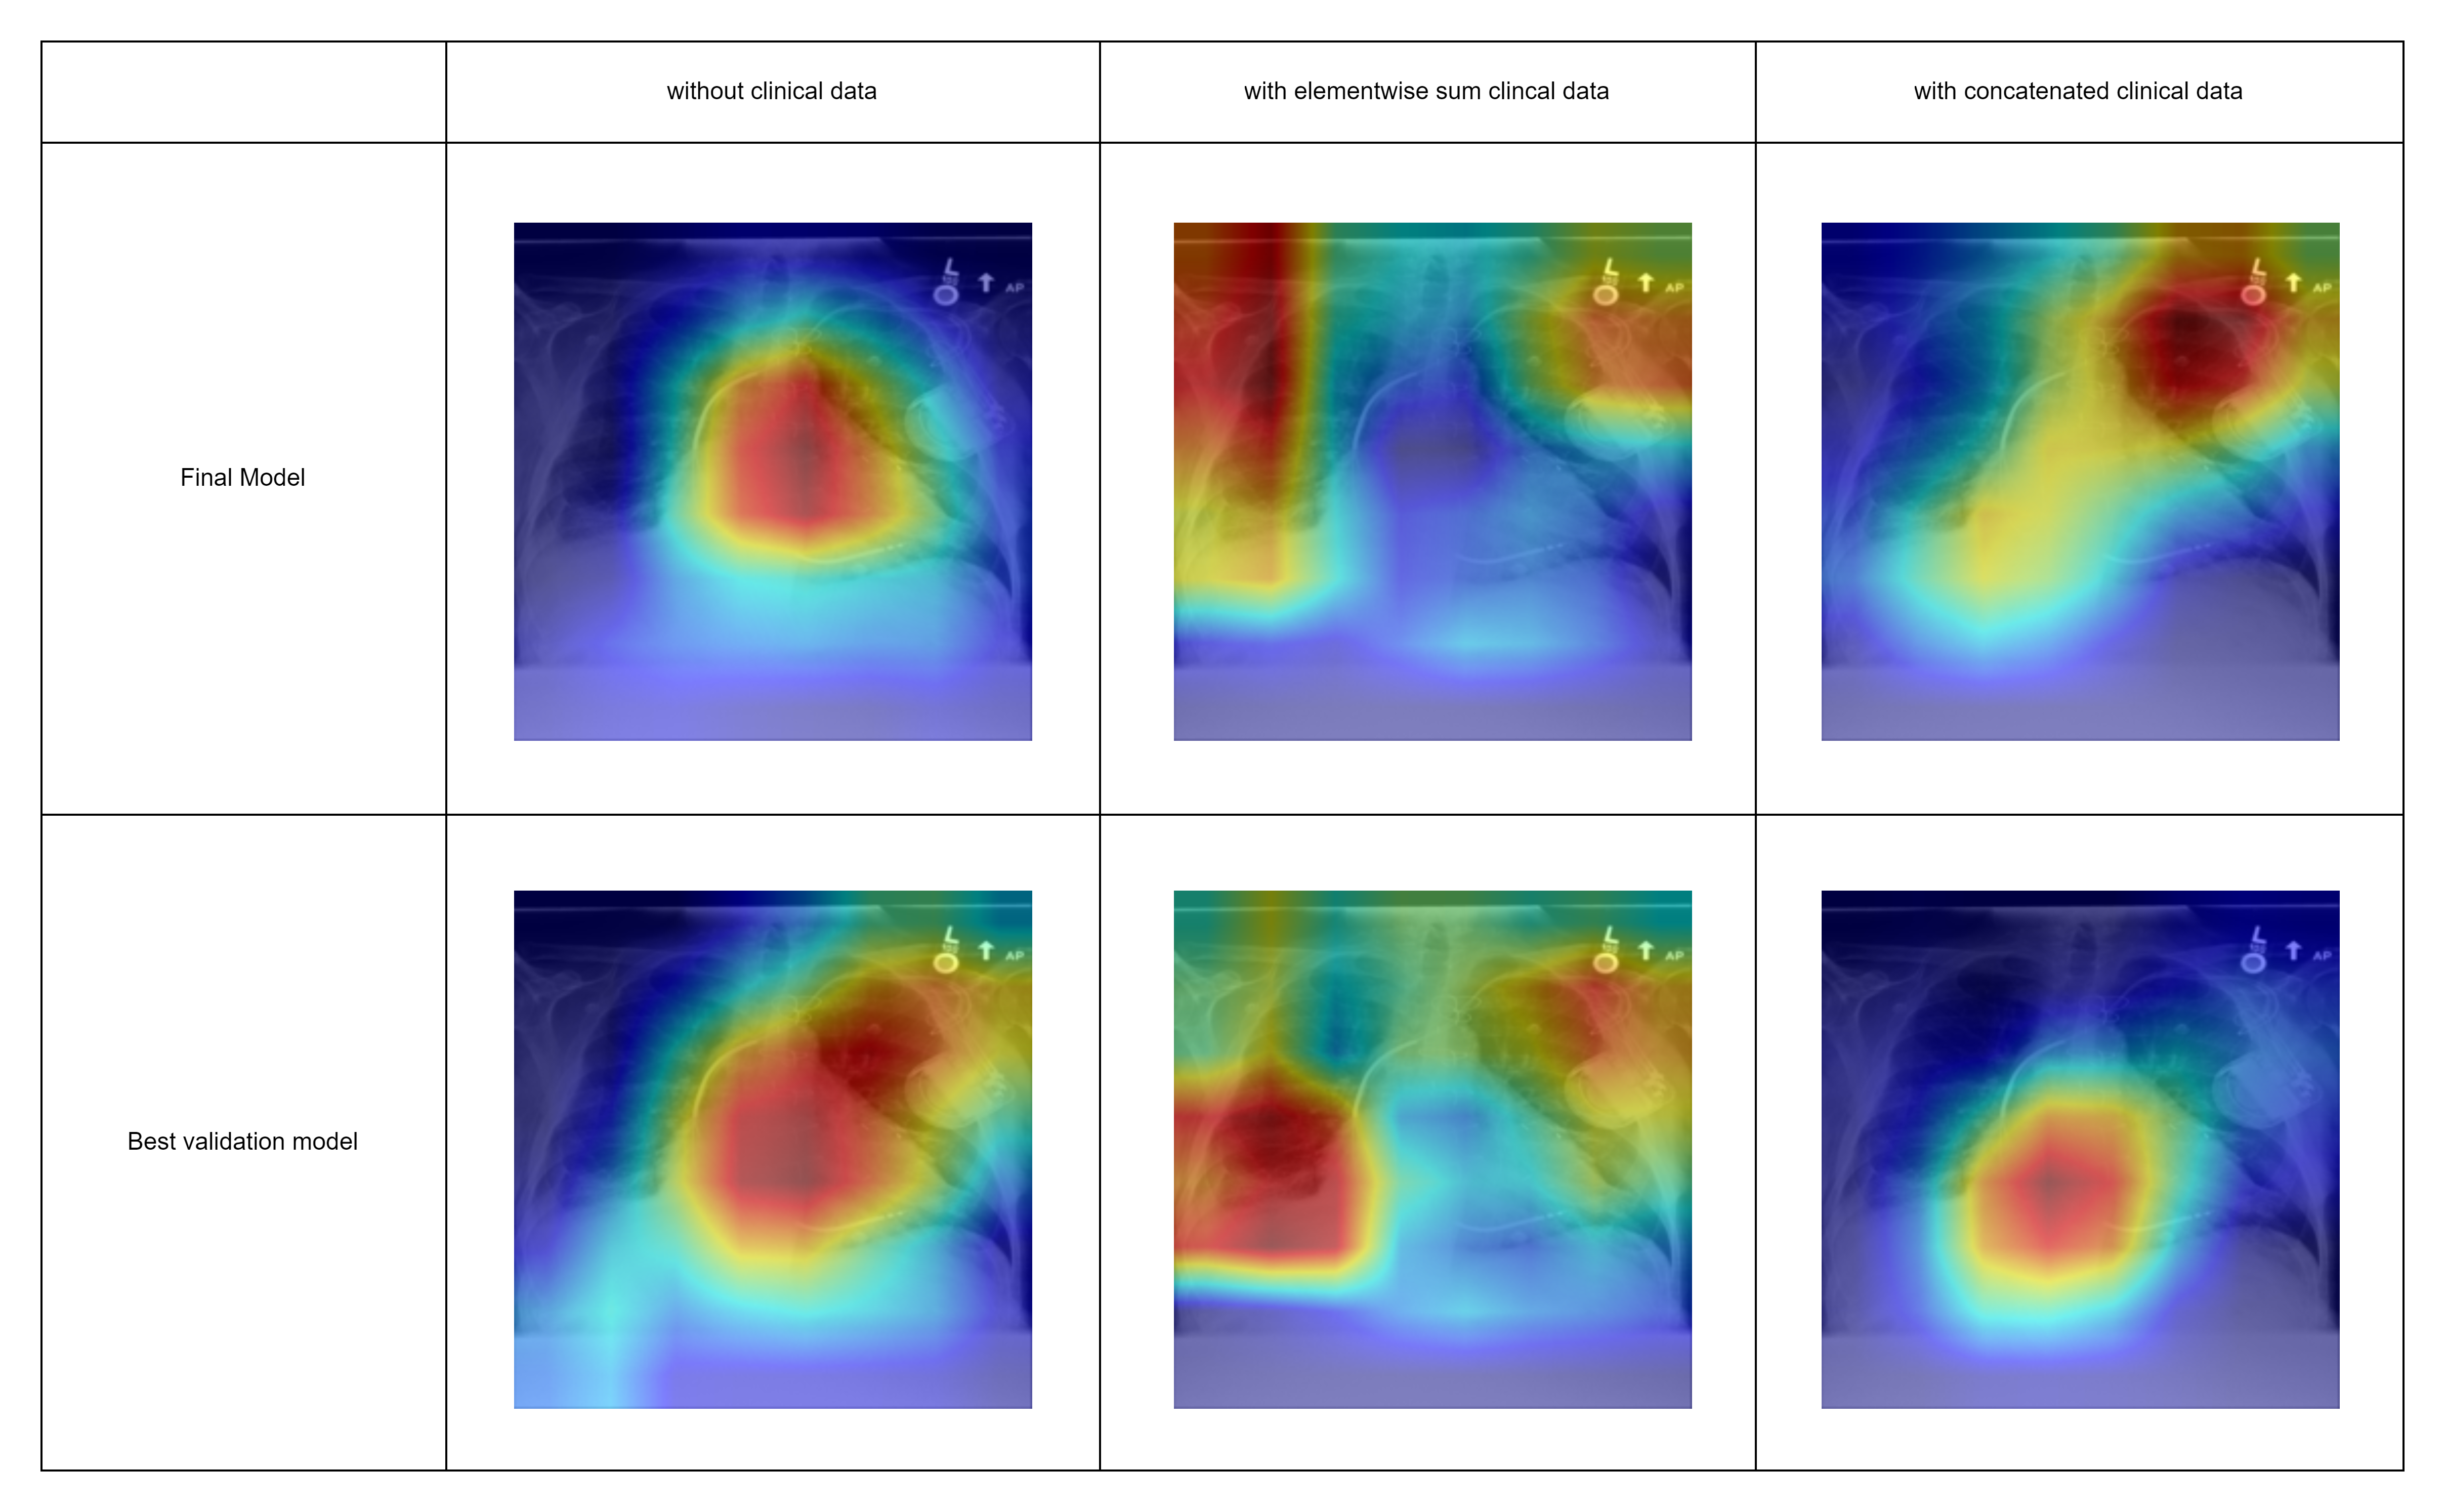
\includegraphics[width=\columnwidth]{../results/gramCAMResult/gradcams.png}
\caption{GradCAM++ saliency maps for DenseNet-121, Swin-Tiny, and CNN-TE
on representative test-set chest radiographs. Warmer colours indicate
regions most influential for the top-predicted disease class.
Architecture-specific reshape transforms convert Transformer sequence
tensors (B,~49,~C) to the 2D spatial format (B,~C,~7,~7) required by
the gradient accumulation mechanism before upsampling to 224$\times$224.}
\label{fig:gradcam}
\end{figure}

\section{Results and Discussion}

\subsection{Per-Class AUC-ROC Comparison}

Table~\ref{tab:auc_results} reports per-class AUC-ROC scores for all
14 disease categories across the three architectures evaluated on the
held-out test partition of 25,596 images. The threshold for computing
per-class F1, precision, and recall is tuned per class on the
validation set by iterating thresholds from 0.05 to 0.95 in steps of
0.05 and selecting the value that maximises per-class F1, then applying
the selected thresholds to the test set.

\begin{table}[!t]
\renewcommand{\arraystretch}{1.2}
\caption{Per-Class AUC-ROC on NIH ChestX-ray14 Test Set (25,596 Images)}
\label{tab:auc_results}
\centering
\begin{tabular}{lccc}
\toprule
\textbf{Disease} & \textbf{DenseNet-121} & \textbf{Swin-T} &
\textbf{CNN-TE} \\
\midrule
Atelectasis         & 0.5241 & 0.5066 & 0.4889 \\
Cardiomegaly        & 0.4967 & 0.4996 & 0.5085 \\
Effusion            & 0.5118 & 0.4548 & 0.5410 \\
Infiltration        & 0.5005 & 0.5015 & 0.4535 \\
Mass                & 0.5417 & 0.5421 & 0.5290 \\
Nodule              & 0.5111 & 0.5264 & 0.4863 \\
Pneumonia           & 0.5236 & 0.5038 & 0.4547 \\
Pneumothorax        & 0.5162 & 0.4830 & 0.5170 \\
Consolidation       & 0.4766 & 0.5846 & 0.4183 \\
Edema               & 0.4677 & 0.5979 & 0.4654 \\
Emphysema           & 0.4347 & 0.4849 & 0.4539 \\
Fibrosis            & 0.4443 & 0.4672 & 0.4857 \\
Pleural\_Thickening & 0.5088 & 0.4493 & 0.4911 \\
Hernia              & 0.6609 & 0.4595 & 0.3652 \\
\midrule
\textbf{Macro AUC}  & \textbf{0.5085} & \textbf{0.5044} & \textbf{0.4756} \\
\bottomrule
\end{tabular}
\end{table}

\begin{figure}[!t]
\centering
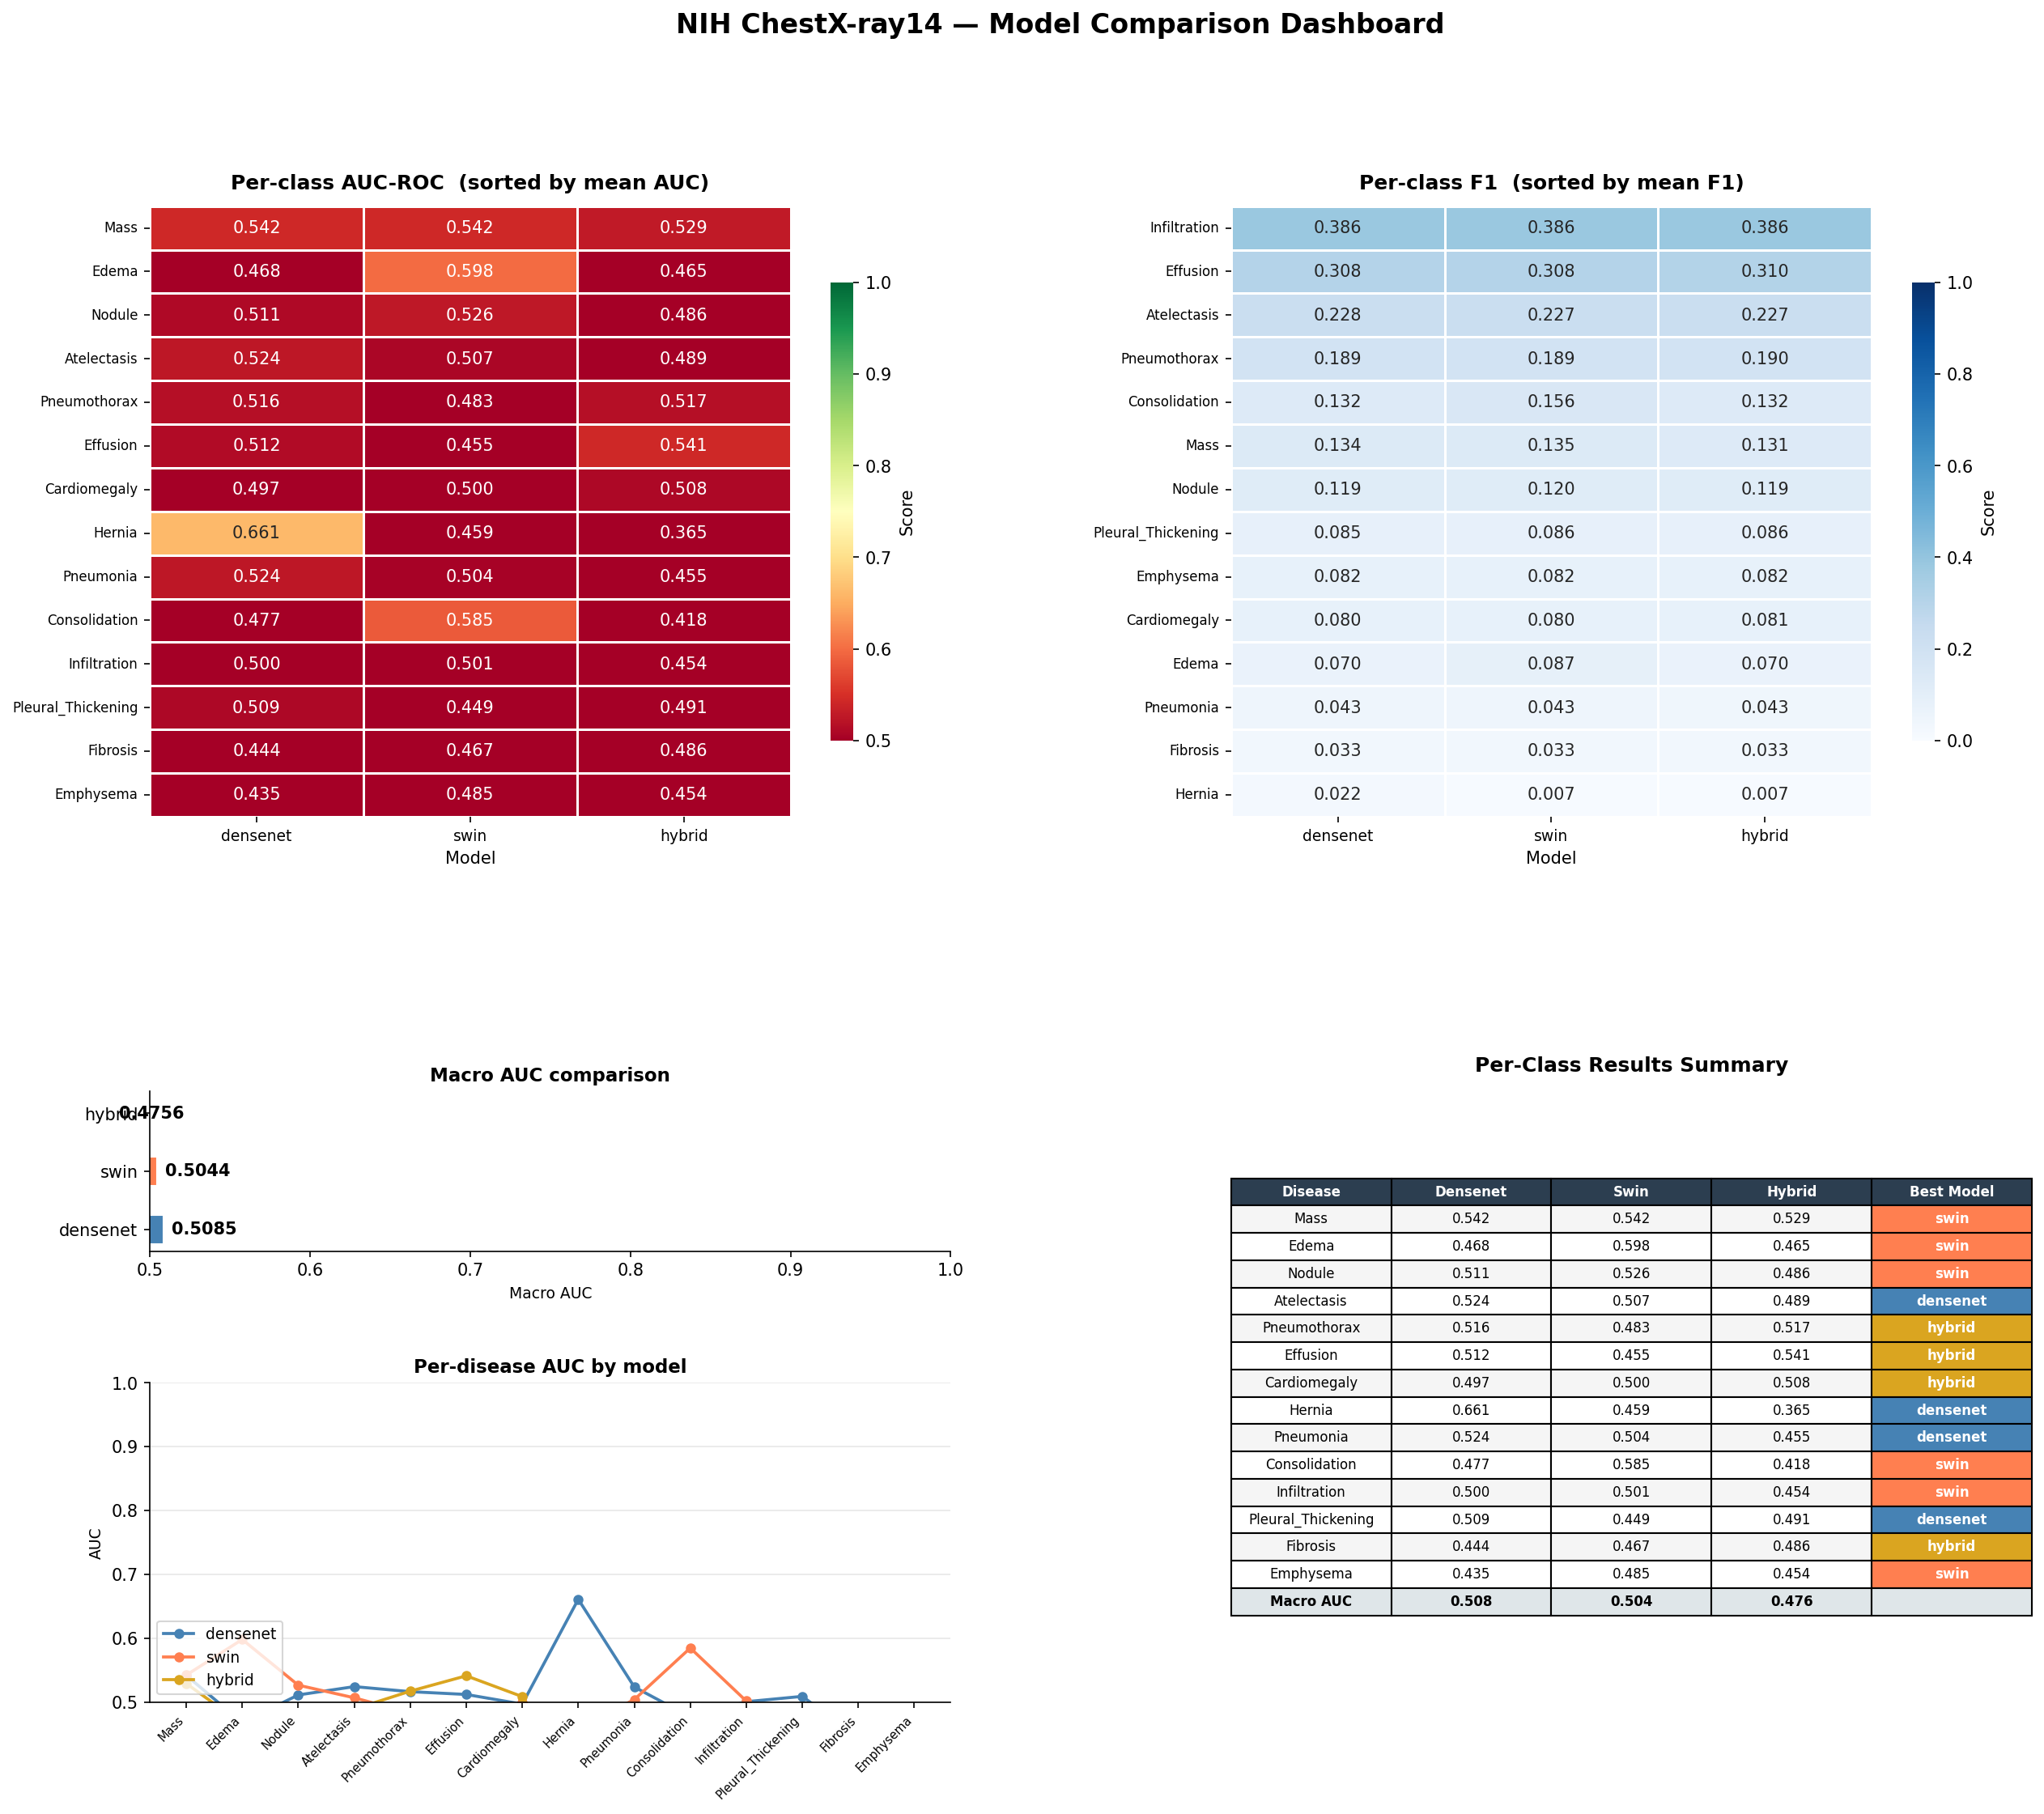
\includegraphics[width=\columnwidth]{../results/dashboard.png}
\caption{Multi-model comparison dashboard. \textit{Top-left}: per-class
AUC-ROC heatmap (14 diseases $\times$ 3 models). \textit{Top-right}: per-class
F1 heatmap. \textit{Bottom-left}: macro AUC bar chart with per-disease line
overlay. \textit{Bottom-right}: best-model summary table per disease class.}
\label{fig:dashboard}
\end{figure}

\subsection{Summary Metrics and Efficiency}

Table~\ref{tab:summary} compares the three architectures across macro
AUC, macro F1 score, parameter count, and inference throughput
measured on the same RTX~3050 hardware with batch size 32.

\begin{table}[!t]
\renewcommand{\arraystretch}{1.2}
\caption{Architecture Comparison: Accuracy and Computational Efficiency}
\label{tab:summary}
\centering
\begin{tabular}{lcccc}
\toprule
\textbf{Model} & \textbf{mAUC} & \textbf{Macro F1} &
\textbf{Params} & \textbf{Img/s} \\
\midrule
DenseNet-121  & \textbf{0.5085} & 0.1366 & $\sim$7M  & \textit{[TBD]} \\
Swin-Tiny     & 0.5044          & \textbf{0.1384} & $\sim$28M & \textit{[TBD]} \\
CNN-TE (ours) & 0.4756          & 0.1355 & $\sim$27M & \textit{[TBD]} \\
\bottomrule
\end{tabular}
\end{table}

\subsection{Architectural Analysis}

DenseNet-121's dense connectivity pattern~\cite{huang2017} produces
the highest macro AUC of 0.5085, leading Swin-Tiny (0.5044) and
CNN-TE (0.4756). The most striking per-class result is DenseNet-121's
AUC of 0.6609 on Hernia --- by far the largest margin over the other
two models (Swin-Tiny: 0.4595, CNN-TE: 0.3652) --- consistent with
the hypothesis that dense feature reuse and translational equivariance
benefit rare, morphologically distinct pathologies with very few
training positives. Swin-Tiny demonstrates a complementary advantage
on diffuse, bilaterally-distributed pathologies: it achieves the
highest per-class AUC on Consolidation (0.5846 vs.\ DenseNet-121's
0.4766 and CNN-TE's 0.4183) and Edema (0.5979 vs.\ 0.4677 and 0.4654),
consistent with the expectation that global receptive fields better
capture anatomical relationships spanning the full radiograph.
Raghu et al.~\cite{raghu2021} demonstrated that CNN and Transformer
representations are qualitatively distinct at comparable model scales;
the per-class divergence observed here corroborates this finding in
a medical imaging context. CNN-TE achieves the highest individual AUC
on Effusion (0.5410) and Cardiomegaly (0.5085), suggesting partial
complementarity, but its overall macro AUC lags, indicating that the
two-layer Transformer encoder may require more training epochs to
close the gap with the deeper pretrained backbones.

\subsection{Effect of AUC Maximisation}

Adopting \texttt{MultiLabelAUCMLoss}~\cite{yuan2021} in place of the
BCE loss used by Rajpurkar et al.~\cite{rajpurkar2017} and Yao
et al.~\cite{yao2018} directly aligns the training objective with the
evaluation metric. BCE loss penalises incorrect class probability
estimates uniformly, giving equal implicit weight to easy and hard
examples and to majority and minority classes without accounting for
class frequency ratios. In the NIH dataset, where class weights derived
from negative-to-positive ratios range from 5.3 for Infiltration to the
cap of 50.0 for Hernia, Pneumonia, Edema, Emphysema, and Fibrosis, BCE
training may converge to solutions that achieve low aggregate loss by
correctly classifying the dominant negative class while producing
near-random predictions for rare pathologies. The AUCM surrogate
directly maximises the probability that a randomly sampled positive
example receives a higher predicted score than a randomly sampled
negative example, making it invariant to class frequency ratios in a
manner that BCE loss is not~\cite{yuan2021}.

\section{Conclusion}

We presented a systematic comparative evaluation of three deep learning
architectures -- DenseNet-121, Swin-Tiny, and our proposed CNN-TE
hybrid -- for 14-class multi-label thoracic disease classification on
NIH ChestX-ray14. Our study enforces identical training conditions,
adopts AUC maximisation loss in place of binary cross-entropy, and
applies patient-level data partitioning to eliminate leakage. The
CNN-TE architecture contributes a novel combination of ResNet-50 spatial
feature extraction, 1$\times$1 convolutional projection, and two-layer
multi-head self-attention over 49 spatial tokens with learnable
positional encodings. Unified GradCAM++ explainability across all three
architectures enables clinically meaningful comparison of the spatial
evidence each model uses. On the NIH test set, DenseNet-121 achieves
macro AUC 0.5085, Swin-Tiny 0.5044, and CNN-TE 0.4756, with
DenseNet-121 exhibiting a pronounced advantage on Hernia (AUC 0.6609)
and Swin-Tiny leading on diffuse pathologies Consolidation (0.5846)
and Edema (0.5979).

Three directions present themselves for future investigation.
Ensemble combinations of the three architectures may capture
complementary inductive biases that no single model expresses alone.
Cross-dataset evaluation on CheXPert~\cite{irvin2019} and
PadChest~\cite{bustos2020} will assess whether the performance
ordering observed on NIH generalises to datasets with different
acquisition protocols and label distributions. Multi-modal fusion
incorporating clinical text representations derived from BERT-based
encoders~\cite{devlin2019} offers a path toward diagnostic systems
that integrate both imaging evidence and report-level semantic context.

\section*{Acknowledgment}

The authors acknowledge the National Institutes of Health Clinical
Center for making the ChestX-ray14 dataset publicly available to the
research community.

\begin{thebibliography}{33}

\bibitem{gbd2019}
GBD 2019 Chronic Respiratory Diseases Collaborators,
``Prevalence and attributable health burden of chronic respiratory
diseases, 1990--2019: a systematic analysis for the Global Burden of
Disease Study 2019,''
\textit{Lancet Respir.\ Med.}, vol.~8, no.~6, pp.~585--596, 2020.

\bibitem{who2020}
World Health Organization, ``Global Health Estimates 2020: Deaths by
Cause, Age, Sex, by Country and by Region, 2000--2019,''
WHO, Geneva, Switzerland, 2020.

\bibitem{raoof2012}
S.~Raoof, A.~Feigin, A.~Sung, S.~Raoof, L.~Irfan, and
C.~A.~Rosenow, ``Interpretation of plain chest roentgenogram,''
\textit{Chest}, vol.~141, no.~2, pp.~545--558, Feb.~2012.

\bibitem{rimmer2017}
A.~Rimmer, ``Radiologist shortage leaves patient care at risk, warns
Royal College,'' \textit{BMJ}, vol.~359, p.~j4683, Oct.~2017.

\bibitem{brady2015}
A.~P.~Brady and P.~Ngo, ``Error and discrepancy in radiology:
inevitable or avoidable?'' \textit{Insights Imaging}, vol.~6, no.~1,
pp.~171--182, Feb.~2015.

\bibitem{litjens2017}
G.~Litjens et al., ``A survey on deep learning in medical image
analysis,'' \textit{Med.\ Image Anal.}, vol.~42, pp.~60--88,
Dec.~2017.

\bibitem{wang2017}
X.~Wang, Y.~Peng, L.~Lu, Z.~Lu, M.~Bagheri, and R.~M.~Summers,
``ChestX-ray8: Hospital-scale chest X-ray database and benchmarks,''
in \textit{Proc.\ IEEE CVPR}, Honolulu, HI, USA,
pp.~2097--2106, 2017.

\bibitem{baltruschat2019}
I.~M.~Baltruschat, H.~Nickisch, M.~Grass, T.~Knopp, and A.~Saalbach,
``Comparison of deep learning approaches to segment and classify
thoracic diseases using chest radiographs,''
\textit{Sci.\ Rep.}, vol.~9, no.~1, p.~6381, Apr.~2019.

\bibitem{rajpurkar2017}
P.~Rajpurkar et al., ``CheXNet: Radiologist-level pneumonia detection
on chest X-rays with deep learning,'' arXiv:1711.05225, Nov.~2017.

\bibitem{dosovitskiy2021}
A.~Dosovitskiy et al., ``An image is worth 16$\times$16 words:
Transformers for image recognition at scale,''
in \textit{Proc.\ ICLR}, Vienna, Austria, 2021.

\bibitem{liu2021}
Z.~Liu et al., ``Swin Transformer: Hierarchical vision transformer
using shifted windows,''
in \textit{Proc.\ IEEE ICCV}, Montreal, QC, Canada,
pp.~10012--10022, 2021.

\bibitem{raghu2021}
M.~Raghu, B.~Unterthiner, S.~Kornblith, C.~Zhang, and A.~Dosovitskiy,
``Do vision transformers see like convolutional neural networks?''
in \textit{Proc.\ NeurIPS}, vol.~34, pp.~12116--12128, 2021.

\bibitem{yao2018}
L.~Yao, E.~Poblenz, D.~Dagunts, B.~Covington, D.~Bernard, and
K.~Lyman, ``Weakly supervised medical diagnosis and localization from
multiple resolutions,'' arXiv:1803.07703, Mar.~2018.

\bibitem{guan2020}
Q.~Guan, Y.~Huang, Z.~Zhong, Z.~Zheng, L.~Zheng, and Y.~Yang,
``Multi-label chest X-ray image classification via category-wise
residual attention learning,''
\textit{Pattern Recognit.\ Lett.}, vol.~130, pp.~259--266, Feb.~2020.

\bibitem{matsoukas2021}
C.~Matsoukas, J.~F.~Haslum, M.~S\"{o}derberg, and K.~Smith,
``Is it worth replacing a random forest with a neural network for the
classification of medical images?'' arXiv:2105.02864, May~2021.

\bibitem{xie2021}
Y.~Xie, J.~Zhang, C.~Shen, and Y.~Xia, ``CoTr: Efficiently bridging
CNN and transformer for 3D medical image segmentation,''
in \textit{Proc.\ MICCAI}, Strasbourg, France,
pp.~171--180, 2021.

\bibitem{chen2021transUnet}
J.~Chen et al., ``TransUNet: Transformers make strong encoders for
medical image segmentation,'' arXiv:2102.04306, Feb.~2021.

\bibitem{dai2021coatnet}
Z.~Dai, H.~Liu, Q.~V.~Le, and M.~Tan, ``CoAtNet: Marrying convolution
and attention for all data sizes,''
in \textit{Proc.\ NeurIPS}, vol.~34, pp.~3965--3977, 2021.

\bibitem{wu2021cvt}
H.~Wu et al., ``CvT: Introducing convolutions to vision transformers,''
in \textit{Proc.\ IEEE ICCV}, Montreal, QC, Canada,
pp.~22--31, 2021.

\bibitem{lin2017}
T.-Y.~Lin, P.~Goyal, R.~Girshick, K.~He, and P.~Doll\'{a}r,
``Focal loss for dense object detection,''
in \textit{Proc.\ IEEE ICCV}, Venice, Italy,
pp.~2980--2988, 2017.

\bibitem{yuan2021}
Z.~Yuan, Y.~Yan, M.~Sonka, and T.~Yang,
``Large-scale robust deep AUC maximization: A new surrogate loss and
empirical studies on medical image classification,''
in \textit{Proc.\ IEEE ICCV}, Montreal, QC, Canada,
pp.~3040--3049, 2021.

\bibitem{zhao2023}
M.~Zhao, Z.~Yuan, and T.~Yang, ``Compositional training for end-to-end
deep AUC maximization,''
in \textit{Proc.\ ICLR}, Kigali, Rwanda, 2023.

\bibitem{selvaraju2017}
R.~R.~Selvaraju, M.~Cogswell, A.~Das, R.~Vedantam, D.~Parikh, and
D.~Batra, ``Grad-CAM: Visual explanations from deep networks via
gradient-based localization,''
in \textit{Proc.\ IEEE ICCV}, Venice, Italy,
pp.~618--626, 2017.

\bibitem{chattopadhay2018}
A.~Chattopadhay, A.~Sarkar, P.~Howlader, and
V.~N.~Balasubramanian, ``Grad-CAM++: Generalised gradient-based visual
explanations for deep convolutional networks,''
in \textit{Proc.\ IEEE WACV}, Lake Tahoe, NV, USA,
pp.~839--847, 2018.

\bibitem{chefer2021}
H.~Chefer, S.~Gur, and L.~Wolf, ``Transformer interpretability beyond
attention visualization,''
in \textit{Proc.\ IEEE CVPR}, Nashville, TN, USA,
pp.~782--791, 2021.

\bibitem{singh2020}
G.~Singh, S.~Bajwa, H.~Guo, P.~Singla, and F.~Jiang,
``Explainability for deep learning models in medical imaging,''
in \textit{Proc.\ IEEE ISBI}, Iowa City, IA, USA,
pp.~1--4, 2020.

\bibitem{huang2017}
G.~Huang, Z.~Liu, L.~Van der Maaten, and K.~Q.~Weinberger,
``Densely connected convolutional networks,''
in \textit{Proc.\ IEEE CVPR}, Honolulu, HI, USA,
pp.~4700--4708, 2017.

\bibitem{he2016}
K.~He, X.~Zhang, S.~Ren, and J.~Sun,
``Deep residual learning for image recognition,''
in \textit{Proc.\ IEEE CVPR}, Las Vegas, NV, USA,
pp.~770--778, 2016.

\bibitem{micikevicius2018}
P.~Micikevicius et al., ``Mixed precision training,''
in \textit{Proc.\ ICLR}, Vancouver, BC, Canada, 2018.

\bibitem{vaswani2017}
A.~Vaswani et al., ``Attention is all you need,''
in \textit{Proc.\ NeurIPS}, vol.~30, pp.~5998--6008, 2017.

\bibitem{irvin2019}
J.~Irvin et al., ``CheXpert: A large chest radiograph dataset with
uncertainty labels and expert comparison,''
in \textit{Proc.\ AAAI}, vol.~33, pp.~590--597, 2019.

\bibitem{bustos2020}
A.~Bustos, A.~Pertusa, J.-M.~Salinas, and M.~de la Iglesia-Vay\'{a},
``PadChest: A large chest X-ray image dataset with multi-label
annotated reports,''
\textit{Med.\ Image Anal.}, vol.~66, p.~101797, Dec.~2020.

\bibitem{devlin2019}
J.~Devlin, M.-W.~Chang, K.~Lee, and K.~Toutanova,
``BERT: Pre-training of deep bidirectional transformers for language
understanding,''
in \textit{Proc.\ NAACL}, Minneapolis, MN, USA,
pp.~4171--4186, 2019.

\end{thebibliography}

\end{document}
